%%%%Select the class of document
\documentclass{amsart} %type/class of article
%\documentclass{article}
%\documentclass{book}
%\documentclass{letter}

%%%%Select packages
\usepackage{amsthm,amsmath,amssymb} %math packages (always include)
\usepackage{geometry} %can be used to modify page dimensions, etc.
\usepackage{graphicx} %figure
\usepackage{float} %figure position in pdf
\usepackage{multirow} %table with multirow
\usepackage[labelfont=rm]{subcaption} %subcaption of figure
\usepackage[numbers]{natbib} %management of bibliography
\usepackage{listings} %use to list command or else in block
\usepackage{xcolor}  %allow to display color
\usepackage{url}
\usepackage{placeins}
\usepackage{algorithm}
\usepackage[noend]{algpseudocode}
%%%%% End Select packages


%%%% Define a style used to display a block of Latex code
\lstdefinestyle{TexStyle}{
language={[LaTeX]TeX},
frame=single,
backgroundcolor=\color{white},
basicstyle=\small\ttfamily,
morekeywords={maketitle,includegraphics},
keywordstyle=\color{blue},  
commentstyle=\color{gray},
stringstyle=\color{black}
}
\definecolor{dkgreen}{rgb}{0,0.6,0}
\definecolor{gray}{rgb}{0.5,0.5,0.5}
\definecolor{mauve}{rgb}{0.58,0,0.82}

\lstset{frame=tb,
	language=C,
	aboveskip=3mm,
	belowskip=3mm,
	showstringspaces=false,
	columns=flexible,
	basicstyle={\small\ttfamily},
	numbers=none,
	numberstyle=\tiny\color{gray},
	keywordstyle=\color{blue},
	commentstyle=\color{dkgreen},
	stringstyle=\color{mauve},
	breaklines=true,
	breakatwhitespace=true,
	tabsize=2
}    


%%%% Set up title page information
\title{CAAM 520: Computational Science II \\
Homework 2.}
\author{Wei Wu}
%\date{\today}
%%%% End Set up title page information


%%% Begin document
\begin{document}

%%%% Write an abstract if needed
%\begin{abstract}
%You can add an abstract at the beginning of the article.
%\end{abstract}

%%%% Make title page
\maketitle

\section{Introduction} 

In this project, we build upon the previous project: we parallelize our linear system solver using MPI. 

\subsection{Mesh Grid Partition}

We partition the mesh grid by the rows, illustrated by the picture below. 

\begin{figure}[!htb]
  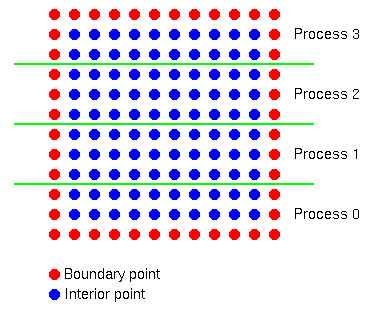
\includegraphics[width=50mm]{grid.jpg}
  \caption{Mesh grid partition}
  \label{fig:boat1}
\end{figure}
\FloatBarrier

However, I made the design decision to only partition the interior nodes.  Let N be the number of interior nodes in a single row, and let s be the number of processors used. I try to divide the interior nodes by rows evenly among all processors. If rm is the remainder of N divided by s, I allocate extra rm rows to processor 0. Two extra rows of ghost nodes, one at the bottom and the other at the top, are allocated for the local u.   

\begin{lstlisting}
	/* 
	Design decision: allocate extra N%size rows to processor 0,
	and N/size + 2 to all other processes. 
	*/  
	int local_row_size = N/size + 2;
	if (rank == 0){
		local_row_size += N%size;
	}
	
	double *local_u = (double*) calloc((local_row_size)*(N+2),sizeof(double));
	double *f = (double*) calloc((local_row_size)*(N+2), sizeof(double));
	double h = 2.0/(N+1);
	
	for (int i = 0; i < N+2; ++i){
		for (int j = 0; j <
			local_row_size; ++j){
			const double x = -1.0 + i*h;
			double y = -1.0 + j*h;
			if (rank > 0)
				y += (rank - 1)*(N/size)*h + (N/size + N%size)*h;
			f[i + j*(N+2)] = sin(PI*x)*sin(PI*y) * h*h;
		}
	}
\end{lstlisting}

\subsection{Parallel weighted Jacobi}
A very high level pseudocode of the parallel weighted Jacobi: 

\begin{algorithm}
	\caption{My algorithm}\label{euclid}
	\begin{algorithmic}[1]
		\Procedure{myAlgo}{$N,tol, size,rank$}
		\While{$global\_res\geq tol$}
		\State Send up unless $rank = size - 1$, then receive from $rank -1$
		\State Send down unless  $rank = 0$, then receive from $rank + 1$
		\State Compute $u\_local$ using weighted Jacobni; compute $local\_res$
		\State Compute $global\_res$
		\EndWhile\label{euclidendwhile}
		\State \textbf{return} $u\_local$
		\EndProcedure
	\end{algorithmic}
\end{algorithm}

The above pseudocode corresponds to the following code snippet: 

\begin{lstlisting}
		/*
		Ghost nodes are stored on 
		u[0,...,N+1] 
		and 
		u[(local_row_size-1)*(N+2),...,(local_row_size)*(N+2)-1]
		Note that for the bottom and top, the exterior nodes will be 
		ghost nodes. 
		*/
		double *unew = (double*)calloc((N+2)*(local_row_size),sizeof(double));
		
		double w = 1.0;
		double invD = 1./4.;  // factor of h cancels out
		
		double global_res2 = 1.0;
		unsigned int iter = 0;
		MPI_Status status;
		while(global_res2>tol*tol){
		
			double local_res2 = 0.0;
			for (int i=0; i<= N+1; ++i){
				/*Send up unless at the top, then receive from below*/
				if (rank < size - 1)
				MPI_Send(&u[i + (local_row_size-2)*(N+2)], 1, MPI_DOUBLE, 
					rank + 1, 0, MPI_COMM_WORLD);
				if (rank > 0)
					MPI_Recv(&u[i], 1, MPI_DOUBLE, rank-1, 0, MPI_COMM_WORLD, &status);
				/*Send down unless at the bottom, then receive from above*/
				if (rank > 0)
					MPI_Send(&u[i + 1*(N+2)], 1, MPI_DOUBLE, 
					rank-1, 1, MPI_COMM_WORLD);
				if (rank < size - 1)
					MPI_Recv(&u[i + (local_row_size-1)*(N+2)], 1, MPI_DOUBLE,
				rank + 1, 1, MPI_COMM_WORLD, &status);
			}
		
		// update interior nodes using Jacobi; does not touch ghost nodes
		// int global_id;
		for(int i=1; i<=N; ++i){
			for(int j=1; j<=local_row_size-2; ++j){
				const int id = i + j*(N+2); // x-index first
				const double Ru = -u[id-(N+2)]-u[id+(N+2)]-u[id-1]-u[id+1];
				const double rhs = invD*(f[id]-Ru);
				const double oldu = u[id];
				const double newu = w*rhs + (1.0-w)*oldu;
				local_res2 += (newu-oldu)*(newu-oldu);
				unew[id] = newu;
			}
		}
		
		for (int i = 0; i < (N+2)*(local_row_size); ++i){
			u[i] = unew[i];
		} 
		
		++iter;
		
		// calcualte global residual
		MPI_Allreduce(&local_res2, &global_res2, 1, MPI_DOUBLE, MPI_SUM,
		MPI_COMM_WORLD);
\end{lstlisting}

\subsection{Debugging}

I did not use dbg to debug. I extensively used printf and return 0 to single out chunks of code. I checked correctness of the program on a small problem with N = 2, just as last time. 

\section{Results on XPS 13 9370}
For a residual $< 1e-6$ , N = 10. The max error and number of iterations stays the same. Depending on the number of processors, the total time could be either higher or lower than using a single processor. See tables belows for some of the results.  
\begin{table}[ht]
	\caption{N = 10, tol = 1e-6} % title of Table
	\centering % used for centering table
	\begin{tabular}{c c c c} % centered columns (4 columns)
		\hline\hline %inserts double horizontal lines
		Num. Processors & Iter & Max Error & Time(s) \\ [0.5ex] % inserts table
		%heading
		\hline % inserts single horizontal line
		1 & 64 & 0.00137 & 0.00137 \\ % inserting body of the table
		2 & 64 & 0.00137 & 0.000769138 \\
		3 & 64 & 0.00137 & 0.003733 \\
		4 & 64 & 0.00137 & 0.000908077 \\
		5 & 64 & 0.00137 & 0.00152731 \\ 
		6 & 64 & 0.00137 & 0.00202286 \\
		7 & 64 & 0.00137 & 0.00161999 \\
		8 & 64 & 0.00137 & 0.14174 \\[1ex] % [1ex] adds vertical space
		\hline %inserts single line
	\end{tabular}
	\label{table:nonlin} % is used to refer this table in the text
\end{table}

\begin{table}[ht]
	\caption{N = 100, tol = 1e-6} % title of Table
	\centering % used for centering table
	\begin{tabular}{c c c c} % centered columns (4 columns)
		\hline\hline %inserts double horizontal lines
		Num. Processors & Iter & Max Error & Time(s) \\ [0.5ex] % inserts table
		%heading
		\hline % inserts single horizontal line
		1 & 4395 & 6.13072e-06 & 0.88749 \\ % inserting body of the table
		2 & 4395 & 6.13072e-06 & 0.635089 \\
		3 & 4395 & 6.13072e-06 & 0.650189 \\
		4 & 4395 & 6.13072e-06 & 0.567912 \\
		5 & 4395 & 6.13072e-06 & 0.609207 \\ 
		6 & 4395 & 6.13072e-06 & 0.589206 \\
		7 & 4395 & 6.13072e-06 & 0.580673 \\
		8 & 4395 & 6.13072e-06 & 0.650094 \\[1ex] % [1ex] adds vertical space
		\hline %inserts single line
	\end{tabular}
	\label{table:nonlin} % is used to refer this table in the text
\end{table}




%%%% End document
\end{document}
